\documentclass[]{article} 
\usepackage{fullpage}
\usepackage{setspace}
\usepackage{hyperref}
\usepackage{graphicx}
\usepackage{booktabs}
\usepackage{fixltx2e}
\usepackage{float}
\usepackage{amsmath,amsthm,amssymb}

\def\SPSB#1#2{\rlap{\textsuperscript{#1}}\SB{#2}}
\def\SP#1{\textsuperscript{{#1}}}
\def\SB#1{\textsubscript{{#1}}}

\doublespacing

\begin{document}

\title{\textbf{Predicting March Madness via Classification } \\ {\Large A Data Mining Approach to Bracketology} }  
\author{Jonathan Pfeil}         
\date{\today}
\maketitle

\vspace{5mm}

\tableofcontents
\newpage

\begin{abstract}
The annual 64-team NCAA Men's Basketball tournament, known as ``March Madness'', is one of the most popular sporting events of the year both in terms of viewership and gambling. Fans and analysts use various strategies while filling out their brackets, ranging from ``gut feelings'' to advanced ranking metrics such as Kenpom and Saragrin ratings. This purpose of this study was to evaluate the effectiveness of classification algorithms in predicting winners of individual basketball games, as well as entire tournament brackets. The motivating hypothesis was that differences in team's play styles may be able to predict the outcome of individual matchups better than just ranking teams according to a statistical model, and that classification algorithms would be able to learn these matchup-specific patterns.
\end{abstract}

\section{Overview and Related Work}
\subsection{Background: March Madness}
The NCAA Men's Division I Basketball Championship, commonly known as ``March Madness'', is a 64-team Men's College basketball tournament held every March. March Madness is one of the most popular sports events of the year, both in terms of viewership and gambling. 52 million viewers tuned in for the tournament last year \cite{inoffice}, and Las Vegas bets exceeded \$100 million \cite{bettingonmadness}. Fans and analysts pride themselves in their abilities to accurately predict the outcomes of games. This has led the massive popularity of ``bracket pools'', where fans submit a bracket predicting the outcome of every one of the 63 games. In 2013, ESPN alone had 8.15 million bracket submissions to its online competition \cite{espnbracketnum}.

Basketball has an enormous amount of individual and team statistics collected and recorded every game. With years of historical NCAA data available, Data Mining techniques can be used to provide quantitative analysis on which teams have the highest probability of success. By applying these principles to each game of the tournament, it is possible to fill out an entire 63-game bracket.

\subsection{Background: Statistical Predictions}
\label{subsec:stat_predictions}

The idea of leveraging data to predict outcomes of sporting events is a subset of a popular field called Sports Data Analysis \cite{sda}. Professional sports teams now employ teams of data scientists to help them make decisions at all levels of the game. Predictive models are now used in choosing when to make player substitutions, surfacing hidden talent in scouting reports, and finding optimal strategies to play against opponents \cite{sda}.

Many attempts have been made to apply Sports Data Analysis principles to NCAA basketball games. Studies such as Schwertman et al. \cite{moreprobmodels} and Boulier and Stekler \cite{seedingpredictors} built models using only team seedings, and found that seeding is a statistically significant predictor of success. More advanced ranking mechanisms popularized by Jeff Sagarin, Ken Pomeroy, Kenneth Massey, and others are derived from a combination of attributes such as home and away wins, winning margin, strength of schedule, and performance against high-ranked teams \cite{predictingmarchmadness}. Nate Silver has experimented with using a linear combination of multiple ranking systems to generate a new, composite ranking system \cite{natesilver}. After a ranking system has been constructed, winners are predicted by just choosing the higher ranked team in a given matchup.

A slightly more complicated system can be used to generate probabilities of each team winning a given game. Instead of just ranking teams, a statistical model can be built to assign each team what is called a ``power rating''. A power rating is a system in which the difference of two teams' ratings yields the point-spread, or expected margin of victory, if the two teams were to play each other \cite{rankingsystems}. Research has been done by Jess Sonas showing that ordinal ranks can be transformed to power ratings via a logarithmic function if a given rating is not a power rating \cite{jeffsonas}. Given a matchup, the power ratings are then subtracted to obtain the point spread. Stern showed that point spreads are normally distributed with $\mu = 0, \sigma = 10.75$ and that the probability of a team winning a matchup is given by the cumulative distribution function $\Phi(Y/\sigma)$ \cite{pointspreadstoprob}. Therefore, given a rating or ranking system, we can generate the probability of victory for each team in a given matchup.

Even though these probabilities are more descriptive than the original models, they suffer from the same basic flaw: in using a well-ordered ranking or rating system to choose the winner, we have ignored matchup-specific information. Differences in teams' play styles may give a worse overall team an advantage over a better overall team when they face each other. For example, a team which has dominated the league through its strong interior defense may not be favored against a small, three-point shooting team, even though they would perform better than their opponent against the rest of the league. With this in mind, the hypothesis of this paper is that more advanced data mining techniques may be able to learn matchup-specific patterns and outperform traditional statistical prediction methods.

\subsection{Background: Data Mining Predictions}

Although classification and regression typically take a back seat to statistical methods in mainstream sports data analysis, research has still been done on the subject. Dragan Miljkovic et al. treated NBA game-outcome prediction as a classification problem, in which each game could be labeled as ``Home Team Victorious'' or ``Away Team Victorious'' \cite{nbapredictions}. By applying a decision tree and a Naive Bayes' classifier, they were able to predict the outcome of NBA games with 67\% success \cite{nbapredictions}.

Research done by Zifan Shi et al. looked at using Machine Learning techniques to predict the outcome of individual NCAA basketball games -- a similar goal to this project. This research used various classification algorithms to try to predict the outcome of individual games throughout a season. The features used in this research fell into two categories: base stats and derived stats. The base stats were just aggregated stats throughout a season (Points Scored, Points Allowed, etc.), while the derived statistics relied on a wealth of statistical basketball knowledge from analysts such as Dean Oliver and Ken Pomery. There were two major takeaways from this research, both of which influenced the way I conducted my research:
\begin{enumerate}
	\item The complexity of the classifier used did not have a major impact on the predictive power. Simple classifiers such as Naive Bayes performed as well as advanced methods such as Artificial Neural Networks. Rather, the success of classifiers was almost entirely dependent on the quality of the features used \cite{ncaaml}. Because of this, I spent most of my effort on this project researching advanced basketball metrics that could be useful as features.

	\item There appears to be a glass ceiling in predictive power in sports data mining. Zifan Shi et al. estimated that the inherent volatility on live sports made it impossible to consistently predict more than 74-75\% of NCAAB games correctly \cite{ncaaml}. Similar findings have been reported in sports data mining applied to soccer, American football, NCAA football, and NBA basketball \cite{ncaaml}. With this in mind, any results showing successful predictions of $>$ 80\% should be a red flag of either over training or of leaking future data into my datasets.
\end{enumerate}
       
\section{Methodology}
Below is a general outline of the methodology used in this project. The details of each step will be expanded upon in the sections afterwards.
\begin{enumerate}
	\item Obtain box-score data for each game played in the 2010-2014 seasons and save it in a postgresql database.

	\item Calculate aggregated and derived stats for each team after each game. These will be used as features in the classification of their next game.

	\item Train game-prediction classifiers by treating each game as a classification problem which gets labeled  as ``Upset'' or ``No Upset'', where ``No Upset'' predicts the higher ranked team to win (according to NCAA's RPI rating) and ``Upset'' predicts the lower ranked team to win.

	\item Recursively apply the trained classifiers to NCAA brackets to make a prediction for each of the 63 games.

	\item Evaluate the success of each classifier.
\end{enumerate}

\section{Data}
\subsection{Data Acquisition}
The NCAA Archive has box-score data available for each of the 27,080 Division-I NCAAB games played in the 2010-2014 seasons, available at \url{http://stats.ncaa.org/team/inst_team_list?division=1&sport_code=MBB}. An example box-score of a game played between Pittsburgh and North Carolina is shown in Figure \ref{fig:ex_box_score}. Highlighted in red shows the stats for each team that would be scraped and saved to a postgresql database.

\begin{figure}[ht]
	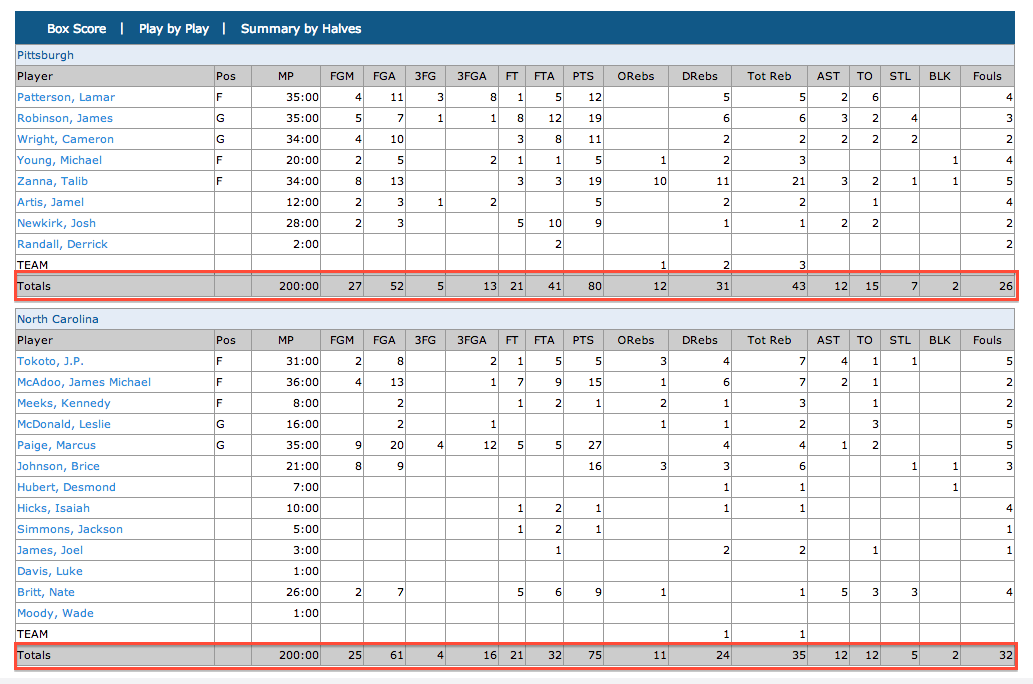
\includegraphics[width=\linewidth]{box_score.png}
	\caption{Example box-score with team stats highlighted}
	\label{fig:ex_box_score}
\end{figure}

\subsection{Base Stats}

For each game, the stats shown in Table \ref{table:base_stats} are saved for each team.

\begin{table}[ht]
\centering
\begin{tabular}{@{}ll@{}}
\toprule
Stat Name                 & Abbreviated Name \\ \midrule
Points                    & PTS              \\
Field Goals               & FG               \\
Field Goal Attempts       & FGA              \\
Three Field Goals         & 3FG              \\
Three Field Goal Attempts & 3FGA             \\
Free Throws               & FT               \\
Free Throw Attempts       & FTA              \\
Offensive Rebounds        & OREB             \\
Defensive Rebounds        & DREB             \\
Total Rebounds            & REB              \\
Assists                   & AST              \\
Turnovers                 & TOV              \\
Steals                    & STL              \\
Blocks                    & BLK              \\
Fouls                     & FOUL             \\ \bottomrule
\end{tabular}
\caption{Table showing team's base stats}
\label{table:base_stats}
\end{table}

Additionally, each team's opponents stats are stored. The base stats of a team's opponent are notated with a superscript as shown in Table \ref{table:opp_base_stats}. 

\begin{table}[ht]
\centering
\begin{tabular}{@{}ll@{}}
\toprule
Stat Name                 & Abbreviated Name \\ \midrule
Points                    & PTS\SP{OPP}              \\
Field Goals               & FG\SP{OPP}               \\
Field Goal Attempts       & FGA\SP{OPP}              \\
Three Field Goals         & 3FG\SP{OPP}              \\
Three Field Goal Attempts & 3FGA\SP{OPP}             \\
Free Throws               & FT\SP{OPP}               \\
Free Throw Attempts       & FTA\SP{OPP}              \\
Offensive Rebounds        & OREB\SP{OPP}             \\
Defensive Rebounds        & DREB\SP{OPP}             \\
Total Rebounds            & REB\SP{OPP}              \\
Assists                   & AST\SP{OPP}              \\
Turnovers                 & TOV\SP{OPP}              \\
Steals                    & STL\SP{OPP}              \\
Blocks                    & BLK\SP{OPP}              \\
Fouls                     & FOUL\SP{OPP}             \\ \bottomrule
\end{tabular}
\caption{Table showing opponent's base stats}
\label{table:opp_base_stats}
\end{table}

\subsection{Basic Derived Stats}

Given the previous Base Stats, we can define the following derived stats for a team and its opponent:

\begin{equation}
	FG\% = \frac{FG}{FGA}
\end{equation}

\begin{equation}
	3FG\% = \frac{3FG}{3FGA}
\end{equation}

\begin{equation}
	FT\% = \frac{FT}{FTA}
\end{equation}


\subsection{Dean Oliver Derived Stats}

In \textit{Basketball on Paper}, author Dean Oliver gave a thorough statistical analysis of NBA basketball teams in an attempt to provide quantitative explanations for team success \cite{basketballonpaper}. My research relies heavily on his work in order to provide predictive features for use in classification; all of the equations below come from \textit{Basketball on Paper}.

In order to normalize statistics w.r.t the ``pace of the game'', we must know the number of possessions that a team had in a game. A possession represents one team controlling the ball; by the rules of basketball, teams necessarily alternate possessions, so a team and its opponent will have the same number of possessions in a given game. Although the number of possessions is not an officially recorded stat, we can estimate it because we know that a possession can only end in one of three ways: a field goal attempt that is not rebounded by the offense, a turnover, or a set of free throws \cite{basketballonpaper}. With this in mind, Dean Oliver has defined the following:

\begin{equation}
	Possessions = FGA - OREB + TOV + 0.4*FTA
\end{equation}

where the 0.4 coefficient represents the proportion of free throws that end a possession.

Given the number of possessions in a game, we can define a team's offensive and defensive efficiencies as the number of points scored and allowed per 100 possessions respectively.

\begin{equation}
	OE = \frac{100*PTS}{Possessions}
\end{equation}

\begin{equation}
	DE = \frac{100*PTS\SP{OPP}}{Possessions}
\end{equation}

We can then derive stats that give us an idea of \textit{how} teams score their points. This will help capture a team's style of play, which we have hypothesized may have strong predictive power in determining the winner a given matchup. We define the following \cite{basketballonpaper}:

\textbf{Scoring Possessions} - Number of possessions in which at least one point is scored
\begin{equation}
	Scoring Possessions = FG + \left[1 - (1- FT\%)^2\right] * 0.4*FTA
\end{equation}

\textbf{Plays} - Number of times a team has the ball (unlike possessions, an offensive rebound marks a new play)
\begin{equation}
	Plays = Possessions + OREB	
\end{equation}

\textbf{Floor Percentage} - Percentage of team's possessions in which at least one point is scored
\begin{equation}
	Floor \% = \frac{Scoring Possessions}{Possessions}
\end{equation}

\textbf{Field Percentage} - Percentage of team's non-foul shot possessions in which at least one point is scored
\begin{equation}
	Field \% = \frac{FG}{FGA - 1.07*\frac{OREB}{OREB+DREB\SP{OPP}}*(FGA-FG)+TOV}
\end{equation}

\textbf{Play Percentage} - Percentage of team's plays in which at least on point is scored
\begin{equation}
	Play\% = \frac{Scoring Possessions}{Plays}
\end{equation}

 Dean Oliver provides a few rules of thumb regarding what these derived stats imply about a team's style of play \cite{basketballonpaper}:

\begin{enumerate}
	\item Teams with high floor percentages and high offensive ratings score very well from the two-point area
	\item Teams with low floor percentages and high offensive ratings score their points by shooting three-pointers
	\item Teams with high field percentages commit few turnovers, get offensive rebounds, and shoot well
	\item Teams with high play percentages and high offensive ratings score well on initial shots, not relying on offensive rebounds to generate points
\end{enumerate}

In addition to these, Dean Oliver relies heavily on the ``Four Factors'' -- four derived stats that he believes captures how effective a team is. They are defined and calculated as follows:

\textbf{Effective Field Goal \%} - Field goal \% adjusted for the importance of three-pointers
\begin{equation}
	eFG\% = \frac{FG = 0.5*3FG}{FGA}
\end{equation}

\textbf{Offensive Rebound \%} - Percentage of offensive rebound opportunities which result in a rebound
\begin{equation}
	OREB\% = \frac{OREB}{OREB + DREB\SP{OPP}}
\end{equation}

\textbf{Turnover Rate} - Percentage of possessions in which a turnover is committed
\begin{equation}
	TOV\% = \frac{TOV}{Possessions}
\end{equation}

\textbf{Free Throw Rate} - Percentage of field goal attempts in which a team draws a foul
\begin{equation}
	FTR = \frac{FTA}{FGA}
\end{equation}

Finally, Dean Oliver provides a way to estimate the win percentage of a team given its statistics. This stat relies on the effect that volatility has on a team's likelihood to win a game. If a team is better than their opponents on average, then being inconsistent will cause them to lose games that they should have won. However, if a team is worse on average, being inconsistent will cause them to win games that they should have lost. This means that the having a large variance in points scored and points allowed brings teams closer to .500, no matter how good they are. With this knowledge, Dean Oliver uses the cumulative distribution function of the standard normal distribution to estimate win percentage as follows:

\begin{equation}
	Win\% = \Phi\left(\frac{FG\SB{mean}-FG\SPSB{OPP}{mean}}{FG\SB{variance}+FG\SPSB{OPP}{variance} - 2*COV(FG, FG\SP{OPP})}\right)
\end{equation}

where $COV(x,y)$ is the covariance of x and y

\subsection{KenPom Derived Attributes}

Ken Pomeroy, author of \url{http://www.kenpom.com}, has expanded upon the work of Dean Oliver in advanced basketball analysis. The equations in this section come from the work he has published on his blog, \url{kenpom.com} \cite{kenpom}.

Pomeroy has advanced the idea of offensive and defensive efficiency under the notion that scoring points against a good defense should be considered more impressive than scoring points against a bad defense, and stopping a good offense should be considered more impressive than stopping a bad offense. This leads to the idea of adjusted offensive and defensive efficiencies. We define them as follows:

\textbf{Adjusted Offensive Efficiency} - An estimate of the offensive efficiency a team would have against the average D-I defense
\begin{equation}
	AdjOE = \frac{OE * OE\SP{LeagueAvg}}{AdjDE\SP{OPP}}
\end{equation}

\textbf{Adjusted Defensive Efficiency} - An estimate of the defensive efficiency a team would have against the average D-I offense
\begin{equation}
	AdjDE = \frac{DE * DE\SP{LeagueAvg}}{AdjOE\SP{OPP}}	
\end{equation}

To avoid the recursive nature of these equations, I used the mean of the opponent's adjusted offensive and defensive efficiencies as of the $(t-1)^{st}$ game of the season to calculate the adjusted offensive and defensive efficiencies in the $t^{th}$ game. This gives the following equations:

\begin{equation}
	{AdjOE}^{t} = \frac{OE * OE\SP{LeagueAvg}}{(AdjDE\SP{OPP})^{t-1}}
\end{equation}
\begin{equation}
	{AdjDE}^{t} = \frac{DE * DE\SP{LeagueAvg}}{(AdjOE\SP{OPP})^{t-1}}
\end{equation}

Since kenpom only makes end-of-season ratings available, I used the above equations to calculate these ratings myself at every point in the season. My end-of-season results matched kenpom's within a constant factor, indicating that the only difference in our calculations were the values used for $OE\SP{LeagueAvg}$ and $DE\SP{LeagueAvg}$.

Finally, kenpom has created a statistic that uses a teams adjusted offensive and defensive ratings to generate an expected winning percentage:

\textbf{Pythagorean Winning \%} - A team's expected winning percentage against an average D-I team
\begin{equation}
	Pyth = \frac{AdjOE^{\gamma}}{AdjOE^{\gamma} + AdjDE^{\gamma}}
\end{equation}

with an empirically derived value of $\gamma = 10.25$

\subsection{Cumulative Stats}

Given the base stats and derived stats for each team in each game, I then calculate a set of Cumulative Stats at each point in the season to be used as features in predicting the result of the next game. For each base stat and derived stat (both of a team and its opponent), I keep track of four new cumulative stats:

\begin{enumerate}
	\item Minimum value in a game up to this point in the season
	\item Maximum value in a game up to this point in the season
	\item Mean value across all games up to this point in the season
	\item Variance of value across all games up to this point in the season
\end{enumerate}

The following formulas are used to update these values iteratively over the course of a season, where $V$ is an arbitrary stat and $V^{t}$ is the value of that stat in the team's $t^{th}$ game of the season:
\begin{equation}
	V\SPSB{t}{min} = min(V\SPSB{t-1}{min}, V\SP{t})
\end{equation}

\begin{equation}
	V\SPSB{t}{max} = max(V\SPSB{t-1}{max}, V\SP{t})
\end{equation}

\begin{equation}
	V\SPSB{t}{mean} = \frac{V\SP{t} + (t-1)V\SPSB{t-1}{mean}}{t}	
\end{equation}

\begin{equation}
	V\SPSB{t}{variance} = \left(\frac{t-2}{t-1}\right)V\SPSB{t-1}{variance} + \frac{\left(V\SP{t}-V\SPSB{t-1}{mean}\right)^{2}}{t}	
\end{equation}

The following base cases are used to complete these recursive definitions:
\begin{equation}
	V\SPSB{1}{min} = V\SP{1}
\end{equation}
\begin{equation}
	V\SPSB{1}{max} = V\SP{1}
\end{equation}
\begin{equation}
	V\SPSB{1}{mean} = V\SP{1}
\end{equation}
\begin{equation}
	V\SPSB{1}{variance} = 0
\end{equation}

\subsection{Rating Systems}
In addition to the Base Stats and Derived Stats listed above, there exists a wealth of knowledge about how good teams are at every point in a season in the form of rating systems. ESPN, sports writers, newspapers, bloggers, etc., all have various statistical methods that they use to generate rating systems, as discussed in Section \ref{subsec:stat_predictions}. Although these may not perform well as individual predictors of success, they may be valuable features in a more complex classification model.

Kenneth Massey, an American sports statistician has compiled and maintained weekly historical team ratings for forty different rating systems \cite{massey}. The ratings used are shown below in Table \ref{table:massey_summary}. These ratings are available publicly at \url{http://www.masseyratings.com/cb/compare.htm}.

\begin{table}[ht]
\centering
\begin{tabular}{@{}ll@{}}
\toprule
System Name         & Abbrev.   \\ \midrule
Associated Press    & AP  \\
Baker Bradley-Terry & BBT \\
Bihl                & BIH \\
BVL Least Squares   & BLS \\
Bobcat              & BOB \\
Colley              & COL \\
D1A Sports          & D1A \\
DeSimone            & DES \\
Donchess Inference  & DII \\
Dokter Entropy      & DOK \\
Dolphin             & DOL \\
ESPN BPI            & EBP \\
Kirkpatrick         & KPK \\
Krach               & KRA \\
Massey              & MAS \\
Moore               & MOR \\
Nolan               & NOL \\
Pugh                & PGH \\
Pigskin             & PIG \\
Pomeroy             & POM \\
\bottomrule
\end{tabular}
\hspace{1em}
\begin{tabular}{@{}ll@{}}
\toprule
System Name         & Abbrev.   \\ \midrule
Pugh Power          & PPR \\
Rewards             & REW \\
RPI                 & RPI \\
RoundTable          & RT  \\
Roundtable BCS      & RTB \\
Rothman             & RTH \\
RT Power            & RTP \\
Sagarin             & SAG \\
Sagarin-Elo         & SE  \\
Self                & SEL \\
Sagarin Predictor   & SP  \\
Snapper's World     & SPW \\
Stanford            & STF \\
The Power Rank      & TPR \\
TeamRankings Pred   & TRP \\
USA Today Coaches   & USA \\
Wilson              & WIL \\
Wiemeyer            & WMR \\
Wobus               & WOB \\
Wolfe               & WOL \\
\bottomrule
\end{tabular}
\caption{Summary of Rating Systems}
\label{table:massey_summary}
\end{table} 


\subsection{Team Feature Summary}

In the above sections, we have looked at 15 base stats, 3 basic derived stats, 13 Dean Oliver stats, and 5 kenpom stats. For each of these\footnote{Excluding $OE$, $DE$, $AdjOE$, and $AdjDE$, since $OE \equiv DE\SP{OPP}$} we also record $V\SP{OPP}$, the opponent's value for the stat (or the amount of that stat that the team has ``allowed''). We then calculate 4 cumulative stats for each of the stats we have at this point: $V\SB{min}, V\SB{max}, V\SB{mean}, V\SB{variance}$. Finally, we add in the 40 ratings obtained from Kenneth Massey. In total this gives us 316 features that describe a team at a given point in the season.

This can be viewed as a vector $\mathbf{x} = \langle x_1, x_2, ..., x_n \rangle$, where $|\mathbf{x}| = 316$

\subsection{Game Features}

All of the features discussed so far have been with respect to a team; however, we ultimately want to run our classification algorithm on games, not teams. Therefore we need a way to generate a feature vector for a game given the two teams participating in it. The strategy taken for this project was to use the difference of the two teams' feature vectors -- specifically, the high-seed's feature vector minus low-seed's feature vector.

\begin{equation}
	\mathbf{g} = \langle g_1, g_2, ..., g_n \rangle = \mathbf{x\SP{high-seed}} - \mathbf{x\SP{low-seed}}
\end{equation}

Since all of the features are positive, we have not lost information about which team's feature value was larger; this is now indicated by the sign of the game feature. Additionally, since the original features were approximately normally distributed, and we know that the sum/difference of normally distributed RVs is normally distributed, the game features are normally distributed as well.

This representation is not without weaknesses, however. It is quite possible that information regarding a team's style of play has been lost in this transformation -- a team shooting more three-pointers than its opponent does not necessarily mean that team is a deep threat. Alternative representations of a game is a potential area for future research.

\section{Preprocessing}
\subsection{Normalization}
\label{subsec:normalization}

Many of the classification algorithms that will be used require that the features roughly follow a standard normal distribution. The game features are already roughly normally distributed; therefore, to transform our features, we only have to remove the mean and scale by the standard deviation.

Let $\mathbf{g_{\mu}}$ be the mean feature vector over all games

Let $\mathbf{g_{\sigma}}$ be a vector whose $i^{th}$ entry is the standard deviation of the $i^{th}$ game feature

Then we can define $\mathbf{g_{c}}$, the normalized version of a given game vector $\mathbf{g}$, elementwise as:
\begin{equation}
	g_{c_i} = \frac{g_i - g_{\mu_i}}{g_{\sigma_i}}
\end{equation}

\subsection{Feature Selection}

27,080 game vectors of length 316 each is a large amount of data -- more data than I hoped to use in classification. Since a large number of games provides helpful training data, I chose to prune the set of features associated with a game. Ideally this would increase the speed of computation by reducing the dimensionality and improve the accuracy by removing features that only serve as noise.

An ANOVA F-test was performed on the set of normalized game vectors, $\left\{ \mathbf{g\SPSB{1}{c}}, \mathbf{g\SPSB{2}{c}}, ..., \mathbf{g\SPSB{N}{c}}\right\}$, against the set of game labels $\left\{ l^1, l^2, ..., l^N \right\}$, $l^i \in \left\{0,1\right\}$ where $0$ represents ``No Upset'' and $1$ represents ``Upset'', in order to remove features with little-to-no correlation with the result of a game.

During classification, the top $k$ features according to the ANOVA test were used, with $k$ determined experimentally. The top 51 features are listed in Table \ref{table:feature_selection}.

\begin{table}[ht]
\centering
\begin{tabular}{@{}ll@{}}
\toprule
Rank & Feature							   \\ \midrule
1  & $PYTH\SB{mean}$          \\ 
2  & $POM$                 \\
3  & $Win\%\SB{mean}$                       \\
4  & $MOR$                 \\
5  & $SAG$                 \\
6  & $Floor\%\SB{mean}$                 \\
7  & $OE\SB{mean}$      \\
8  & $Field\%\SB{mean}$                 \\
9  & $RPI$                 \\
10 & $Play\%\SB{mean}$                  \\
11 & $AdjOE\SB{mean}$ \\
12 & $Floor\%\SPSB{OPP}{mean}$              \\
13 & $DE\SB{mean}$      \\
14 & $Play\%\SPSB{OPP}{mean}$               \\
15 & $AdjDE\SB{mean}$ \\
16 & $Field\%\SPSB{OPP}{mean}$              \\
17 & $Floor\%\SB{max}$                  \\
\bottomrule
\end{tabular}
\hspace{1em}
\begin{tabular}{@{}ll@{}}
\toprule
Rank & Feature							   \\ \midrule
18 & $FG\%\SB{mean}$                    \\
19 & $PTS\SB{mean}$                        \\
20 & $Scoring Possessions\SB{mean}$       \\
21 & $Field\%\SB{max}$                  \\
22 & $eFG\%\SB{mean}$         \\
23 & $OE\SB{max}$       \\
24 & $Scoring Possessions\SPSB{OPP}{mean}$    \\
25 & $PTS\SPSB{OPP}{mean}$                     \\
26 & $FG\SB{mean}$                         \\
27 & $DE\SB{min}$       \\
28 & $AST\SPSB{OPP}{mean}$                     \\
29 & $OE\SB{min}$       \\
30 & $Ply\%\SPSB{OPP}{min}$                \\
31 & $Floor\%\SPSB{OPP}{min}$               \\
32 & $AST\SB{mean}$                        \\
33 & $AdjDE\SB{min}$  \\
34 & $Floor\%\SB{min}$                  \\
\bottomrule
\end{tabular}
\hspace{1em}
\begin{tabular}{@{}ll@{}}
\toprule
Rank & Feature							   \\ \midrule
35 & $AdjOE\SB{min}$  \\
36 & $FG\%\SPSB{OPP}{mean}$                 \\
37 & $eFG\%\SPSB{OPP}{mean}$      \\
38 & $Play\%\SB{max}$                   \\
39 & $REB\SPSB{OPP}{mean}$                     \\
40 & $Field\%\SPSB{OPP}{min}$               \\
41 & $FG\SPSB{OPP}{mean}$                      \\
42 & $Field\%\SB{min}$                  \\
43 & $PTS\SPSB{OPP}{min}$                      \\
44 & $DREB\SPSB{OPP}{mean}$                \\
45 & $Play\%\SB{min}$                   \\
46 & $Scoring Possessions\SPSB{OPP}{min}$     \\
47 & $OREB\%\SPSB{OPP}{mean}$     \\
48 & $PTS\SB{min}$                         \\
49 & $Field\%\SPSB{OPP}{max}$               \\
50 & $Pay\%\SPSB{OPP}{max}$                \\ 
51 & $AST\SB{max}$                \\ \bottomrule
\end{tabular}
\caption{Summary of Feature Selection}
\label{table:feature_selection}
\end{table}

As we would expect, popular ranking systems and derived possession-based statistics are the most predictive stats. The least predictive stats are all variances of base or derived stats.

\section{Classification}
\subsection{5-fold cross validation methodology}
\label{subsec:five_fold}

The methodology used for testing the classification algorithms is as follows:

\begin{enumerate}
	\item Let $\mathbf{G}$ be the set of game vectors $\mathbf{g}$, each of which is composed of the top $k$ selected features. Let $\mathbf{l} = \left\{l_1, l_2, ..., l_N\right\}$ be the set of labels corresponding to game outcomes
	\item Transform each $\mathbf{g} \in \mathbf{G}$ to a corresponding $\mathbf{g_c}$ via the normalization procedure described in Section \ref{subsec:normalization}, generating a new set $\mathbf{G_c}$
	\item Partition ${\mathbf{G_c}}$ into 5 subsets $\mathbf{G_c} = \left\{ \mathbf{G_{c_1}}, \mathbf{G_{c_2}}, \mathbf{G_{c_3}}, \mathbf{G_{c_4}}, \mathbf{G_{c_5}}\right\}$ for use in 5-fold cross validation.
	\item For each $\mathbf{G_{c_i}} \in \mathbf{G_c}$
	\begin{enumerate}
		\item Train the classifier with $\mathbf{G_{c}} - \mathbf{G_{c_i}}$ as the training set
		\item Predict labels $\mathbf{m} = \{m_1, m_2, ..., m_N\}$ for the test data set $\mathbf{G_{c_i}}$
		\item Calculate the classification success via
			\begin{equation}
				success = \frac{\# correct predictions}{\# predictions}\\
			\end{equation}
			\begin{equation}
				success = \frac{\left\vert\left\{m_i | l_i = m_i \right\}\right\vert}{\left\vert\textbf{m}\right\vert}
			\end{equation}
	\end{enumerate}
	\item Take the weighted mean of each partition's success, according to how many elements were in it
\end{enumerate}

\subsection{Classifiers}

The following classifiers were tested:
\begin{enumerate}
	\item Baseline classifier -- Always picks the favorite to win
	\item Naive Bayes classifier
	\item Decision Tree
	\item Random Forest
	\item Support Vector Machine -- Radial Basis Function
	\item Support Vector Machine -- Linear
	\item Artificial Neural Network
	\item Linear Regression -- Predict point differential of high-seed score - low-seed score. If positive return ``No Upset'' else return ``Upset''
\end{enumerate}

\subsection{Full Season Results}

The results in this section come from are the result of trying to classify every game\footnote{This excludes the first 2 games played by each game each season. This is because cumulative stats don't make sense this early in the season.} in the data set via the methodology discussed in Section \ref{subsec:five_fold}, and a $k$-value of 50.

\begin{table}[ht]
\centering
\begin{tabular}{@{}ll@{}}
\toprule
Classifier        & Accuracy \\ \midrule
Baseline          & 66.30\%  \\
Naive Bayes       & 65.92\%  \\
Decision Tree     & 70.93\%  \\
SVM -- RBF        & 71.39\%  \\
SVM -- Linear     & 68.92\%  \\
Neural Net        & 70.96\%  \\
Linear Regression & 64.92\%  \\ \bottomrule
\end{tabular}
\caption{Full Season Classification Accuracies}
\label{table:full_season_classification}
\end{table}

\subsection{Piecewise Classification}
\label{subsec:piecewise}

Intuitively, it makes sense that a feature's predictive power may not remain constant throughout a season. We would expect that early in the season, rankings would be more important (since there only a few games of cumulative stats), but by the end of the season the more advanced computed statistics would be powerful predictors. With this hypothesis, I tried training classifiers on small windows throughout the season, rather than once over the entire season. The results of this are shown in Figures \ref{fig:piecewise} \& \ref{fig:piecewise_zoom} with the average accuracies shown in Table \ref{table:piecewise_classification}.

\begin{figure}[ht]
	\centering
	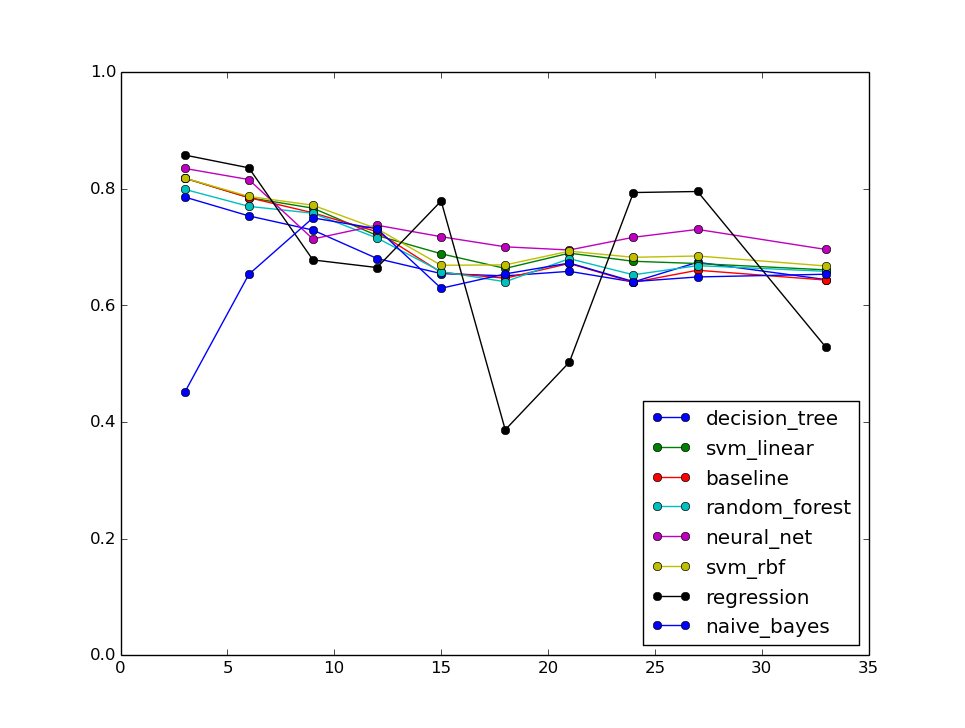
\includegraphics[width=.65\linewidth]{piecewise_classifier.png}
	\caption{Piecewise Classifier}
	\label{fig:piecewise}
\end{figure}

\begin{figure}[ht]
	\centering
	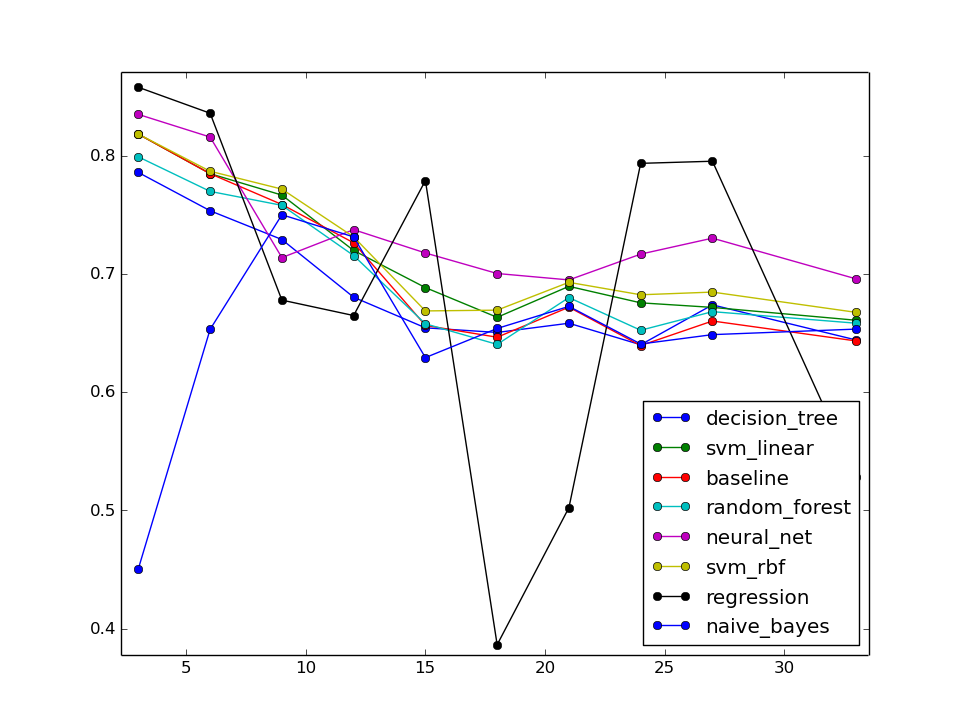
\includegraphics[width=.65\linewidth]{piecewise_classifier_zoom.png}
	\caption{Piecewise Classifier Zoomed}
	\label{fig:piecewise_zoom}
\end{figure}

\begin{table}[ht]
\centering
\begin{tabular}{@{}ll@{}}
\toprule
Classifier        & Accuracy \\ \midrule
Baseline          & 66.30\%  \\
Naive Bayes       & 64.83\%  \\
Decision Tree     & 68.71\%  \\
SVM -- RBF        & 71.73\%  \\
SVM -- Linear     & 71.40\%  \\
Neural Net        & 72.37\%  \\
Linear Regression & 68.21\%  \\ \bottomrule
\end{tabular}
\caption{Piecewise Classification Accuracies}
\label{table:piecewise_classification}
\end{table}

Although the performance of Naive Bayes and the Decision Tree both dropped due to weak early season results, the classifier accuracies went up in general. Most notably, the neural networks were able to achieve a season-wide accuracy of 72.37\%, approaching the glass ceiling estimated in \cite{ncaaml}.

\subsection{Bracket Prediction}

The results in Section \ref{subsec:piecewise} support my hypothesis that the importance of a given feature varies over the course of a season. Because my goal is to predict tournament success (and tournament's occur at the end of a season), the training data will only come from the end of seasons; specifically, I will exclude everything before a team's $q^{th}$ game of the season, where $q$ is an experimentally derived integer. To predict a given season $y$'s bracket, all games played in $\{2010, 2011, 2012, 2013, 2014\}$ - $y$ that were at least the $q^{th}$ game of the season for both teams involved were used as a training set. The success of a bracket prediction was measured in two ways:
\begin{enumerate}
	\item The accuracy formula presented in Section \ref{subsec:five_fold}
	\item ESPN's bracket scoring formula shown below, where $\mathbf{m}$ is the set of predicted labels, $\mathbf{l}$ is the set of correct labels, and $Round(m_i)$ is the round of the tournament that the predicted game was played in (first round = 1, second round = 2, ..., championship round = 6). This formula gives a fixed amount of 320 points to each round, with the points distributed evenly across the games played in that round.
	\begin{equation}
		u(\mathbf{m}, \mathbf{l}) = 10*\sum_{m_i=l_i}2^{Round(m_i) - 1}
	\end{equation}
\end{enumerate}

The bracket-prediction results are summarized in \ref{table:bracket_summary}. The full season-by-season results are shown in Table \ref{table:bracket_prediction}. The propagated error of predicting incorrect winners in early rounds necessarily means that the accuracy percentages will drop from when we were only looking at individual games. This is reflected in the baseline falling from 66.30\% to 40.00\%.

\begin{table}[ht]
\centering
\begin{tabular}{@{}lll@{}}
\toprule
   Classifier           & Accuracy & ESPN Score \\ \midrule
   Baseline             & 40.00\%         & 368           \\
   Naive Bayes          & 32.70\%         & 260           \\
   Decision Tree        & 39.05\%         & 340           \\
   Random Forest        & 44.45\%         & 410           \\
   SVM -- RBF           & 45.40\%         & 370           \\
   SVM -- Linear        & 45.40\%         & 456           \\
   Lin. Reg.            & 40.00\%         & 368           \\
   Neural Net           & 48.57\%         & 474           \\
\bottomrule
\end{tabular}
\caption{Average Bracket Prediction Results}
\label{table:bracket_summary}
\end{table}

\begin{table}[ht]
\centering
\begin{tabular}{@{}llll@{}}
\toprule
Year & Classifier           & Accuracy & ESPN Score \\ \midrule
2010 & Baseline             & 46.03\%         & 540           \\
     & Naive Bayes          & 26.98\%         & 180           \\
     & Decision Tree        & 39.38\%         & 350           \\
     & Random Forest        & 55.56\%         & 650           \\
     & SVM -- RBF           & 49.20\%         & 380           \\
     & SVM -- Linear        & 53.97\%         & 580           \\
     & Lin. Reg.            & 46.03\%         & 540           \\
     & Neural Net           & 57.14\%         & 670           \\ \midrule
2011 & Baseline             & 30.16\%         & 200           \\
     & Naive Bayes          & 31.75\%         & 210           \\
     & Decision Tree        & 38.10\%         & 310           \\
     & Random Forest        & 41.27\%         & 310           \\
     & SVM -- RBF           & 39.68\%         & 280           \\
     & SVM -- Linear        & 39.68\%         & 290           \\
     & Lin. Reg.            & 30.16\%         & 200           \\
     & Neural Net           & 47.62\%         & 390           \\ \midrule
2012 & Baseline             & 26.98\%         & 180           \\
     & Naive Bayes          & 34.92\%         & 250           \\
     & Decision Tree        & 38.10\%         & 390           \\
     & Random Forest        & 41.27\%         & 330           \\
     & SVM -- RBF           & 38.10\%         & 310           \\
     & SVM -- Linear        & 33.33\%         & 400           \\
     & Lin. Reg.            & 26.98\%         & 180           \\
     & Neural Net           & 44.44\%         & 440           \\ \midrule
2013 & Baseline             & 47.62\%         & 410           \\
     & Naive Bayes          & 34.92\%         & 380           \\
     & Decision Tree        & 33.33\%         & 260           \\
     & Random Forest        & 36.51\%         & 350           \\
     & SVM -- RBF           & 46.03\%         & 410           \\
     & SVM -- Linear        & 46.03\%         & 450           \\
     & Lin. Reg.            & 47.62\%         & 410           \\
     & Neural Net           & 42.86\%         & 430           \\ \midrule
2014 & Baseline             & 49.21\%         & 510           \\
     & Naive Bayes          & 34.92\%         & 280           \\
     & Decision Tree        & 46.03\%         & 390           \\
     & Random Forest        & 47.62\%         & 410           \\
     & SVM -- RBF           & 53.97\%         & 470           \\
     & SVM -- Linear        & 52.97\%         & 560           \\
     & Lin. Reg.            & 49.21\%         & 510           \\
     & Neural Net           & 50.79\%         & 440           \\
\bottomrule
\end{tabular}
\caption{Full Bracket Prediction Results}
\label{table:bracket_prediction}
\end{table}

\section{Conclusion}
\subsection{Analysis of Results}

Looking at the results listed in Tables \ref{table:bracket_summary} \& \ref{table:bracket_prediction} we see results that are approximately in line with our regular season predictions. The Naive Bayes classifier still performs worse than the baseline, and the Decision Tree and Linear Regression perform about the same as the baseline. The Random Forest, SVM -- RBF, SVM -- Linear, and Artificial Neural Network classifiers all performed substantially better than the baseline both in terms of the percentage of games predicted correctly and the ESPN bracket score. 

Unlike in the work done by \cite{ncaaml}, the more advanced classification algorithms vastly outperformed the more simplistic models. Perhaps this is because the strong linear dependence between many of the derived attributes; applying principal component analysis before classifying may be able to improve the performance of the simpler models.

\subsection{Future Work}

The hypothesis inspiring this research was that differences in team's play styles may be able to predict the outcome of individual matchups better than just ranking teams according to a statistical model. While the above results show that more advanced classification algorithms were able to substantially outperform the baseline prediction method of always choosing the high-seed, there is still room for improvement. It is unclear whether or not accumulated end-of-game stats have a fine enough granularity to truly capture \textit{how} a team plays. For example, the 2014 Creighton Bluejays ran almost all of their offense through small forward Doug McDermott; McDermott took 37\% of the teams shots \cite{kenpom}. This is a defining characteristic of the Creighton offense, and yet it wouldn't be captured in the box-score data that was used for this project.

A future project then, is to look at a more granular data source. In addition to the box-scores used for this project, the NCAA Archive hosts play-by-play data describing each possession in a given game. By applying data mining techniques to this data set, we may be able to create a more informative description of \textit{how} a given team plays.

\begin{figure}[ht]
	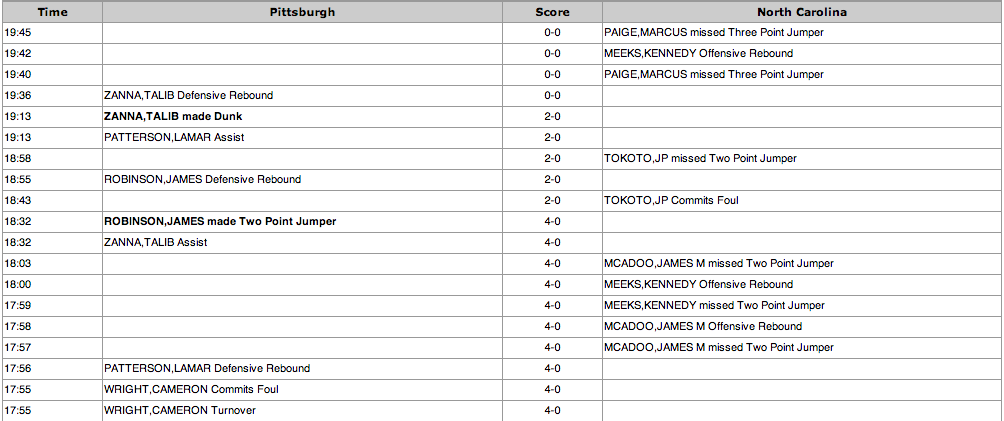
\includegraphics[width=\linewidth]{play_by_play.png}
	\caption{Example play-by-play data}
	\label{fig:ex_play_by_play}
\end{figure}

\clearpage
\newpage
\bibliographystyle{ieeetr} 
\section{Bibliography}     
\begin{thebibliography}{8}
	\bibitem{inoffice} L. Petrecca, ``March Madness in the office: Work comes in second,'' USA TODAY, 3/15/2012.[Online]. \url{http://usatoday30.usatoday.com/money/workplace/story/2012-03-09/march-madness-ncaa-workplace/53538598/1}.

	\bibitem{bettingonmadness}Denny Lee.``Betting on March's Madness." New York Times: F.1. 2005. Print.

	\bibitem{espnbracketnum} D. Haar, ``How Many ESPN.com Brackets Got All Four Right? Very Few," Hartford Courant,
	4/1/2013.[Online]. \url{http://courantblogs.com/dan-haar/how-many-espn-com-brackets-got-all-four-right-very-few/}.

	\bibitem{sda} Schumaker, R., Solieman, O., Chen, H. ``Sports data mining. Springer'', 2010.

	\bibitem{moreprobmodels} Schwertman, Neil C., Kathryn L. Schenk, and Brett C. Holbrook. ``More Probability Models for the NCAA Regional Basketball Tournaments." The American Statistician 50.1 (1996): 34-8. Print.

	\bibitem{seedingpredictors} Boulier, Bryan L., and H. O. Stekler.``Are Sports Seedings Good Predictors?: An Evaluation." International Journal of Forecasting 15.1 (1999): 83-91. Print.

	\bibitem{highseedbetter} Jacobson, S. H., and King, D.M. (2009).``Seeding in the NCAA Men’s Basketball Tournament: When is a Higher Seed Better'', The Journal of Gambling Business and Economics, 3, 63-87.

	\bibitem{predictingmarchmadness} Toutkoushian, Emily. ``Predicting March Madness: A Statistical Evaluation of the Men's NCAA Basketball Tournament." 2011. Print.

	\bibitem{natesilver} N. Silver, ``How We Made Our N.C.A.A. Picks," FiveThirtyEight -- The New York Times, 3/14/2011.[Online]. \url{http://fivethirtyeight.blogs.nytimes.com/2011/03/14/how-we-made-our-n-c-a-a-picks/}.

	\bibitem{nbapredictions} Miljkovic, D., Gajic, L., Kovacevic, A., Konjovic, Z.,``The use of data mining for basketball matches outcomes prediction'', IEEE 8th International Symposium on intelligent and informatics, Subotica, Serbia, 2010, pp.309-312.

	\bibitem{rankingsystems} Sorensen, S. P., ``An Overview of Some Methods For Ranking Sports Teams'', \url{http://www.phys.utk.edu/sorensen/ranking/}

	\bibitem{pointspreadstoprob} Stern H. (1991) ``On the Probability of Winning a Football Game'', The American Statistician, 45, 179-183.

	\bibitem{jeffsonas} Jess Sonas, ``EXTRA DATA - Sagarin Predictive Ratings'', Kaggle, 2/24/14. [Online]. \url{http://www.kaggle.com/c/march-machine-learning-mania/forums/t/6767/extra-data-sagarin-predictive-ratings}

	\bibitem{ncaaml} Shi, Zifan et al. ``Predicting NCAAB match outcomes using ML techniques - some results and lessons learned''. 14 Oct, 2013. arxiv.org.

	\bibitem{basketballonpaper} Dean Oliver. \textit{Basketball on Paper}. Brassey’s, Inc., 2002.

	\bibitem{kenpom} Ken Pomery, ``the kenpom.com blog'' [Online]. \url{http://www.kenpom.com}

	\bibitem{massey} Kenneth Massey, ``College Basketball Ranking Composite'', Massey Ratings [Online]. \url{http://www.masseyratings.com/cb/compare}
	
\end{thebibliography}

\end{document}